\documentclass[11pt]{amsart}
\usepackage{cite}
\usepackage{lmodern}
\usepackage{graphicx}
\usepackage[utf8]{inputenc}

\title{Assignment 1}
\begin{document}

\maketitle

\section*{1.}

We'll use the following notation: '$pos$' for test being positive, '$neg$' for test being negative, '$hiv$' for patient to have HIV and '$\neg hiv$' for the patient not to have HIV.

Priors

$P(pos \mid hiv) = \frac{998}{1000}$ $P(neg \mid hiv) = \frac{2}{1000}$

$P(pos \mid \neg hiv) = \frac{1}{1000}$ $P(neg \mid \neg hiv) = \frac{999}{1000}$

$P(hiv) = \frac{1}{10000}$ $P(\neg hiv) = \frac{9999}{10000}$.

Let's calculate the marginal probability $P(pos)$

\begin{equation*}
    \begin{aligned}
        P(pos) &= P(pos \mid hiv)P(hiv) + P(pos \mid \neg hiv)P(\neg hiv) \\
               &= \frac{1}{1000}\frac{9999}{10000} + \frac{998}{1000}\frac{1}{10000} \\
               &= 0.0010997
    \end{aligned}
\end{equation*}

Now we can just use the Bayes rule

\begin{equation*}
    \begin{aligned}
        P(hiv \mid pos)
        &= \frac{P(pos \mid hiv)P(hiv)}{P(pos)} \\
        &= \frac{\frac{998}{1000}\frac{1}{10000}}{0.0010997} \\
        &\approx 0.091
    \end{aligned}
\end{equation*}

\section*{2.}
\subsection*{Dicing with the uncertainty}

Epistemic uncertainty definitely makes sense. It's all around us. For example let's say that you want to know how many hair are there growing in queen Elizabeth's head. Certainly you can't just go there, rip them off her head one by one and count them - so you have to estimate.

Aleatory uncertainty is a more complex concept. How do you know when something is truly aleatory? Maybe some random fluctuations in quantum theory? But on the other hand, that could be also just lack of knowledge. It's really difficult to justify if something is truly random or just lack of our knowledge. However, in our daily lives aleatory uncertainty definitely exists: when throwing a fair die it's definitely impossible for one to calculate what the outcome will be while the die is in the air. But does the same apply in science? It's not hard to imagine a computer program that takes input of a flying die as input and the output is the result. Maybe not right now, but in the future definitely.

On the practical side, it's not possible to dive deep enough in data analysis to get rid of all the epistemic uncertainty. To estimate some data related to for example the whole population on earth it's not possible to go and ask everyone and get the true data - we have to take a sample and estimate the population data from the sample. I think this is a good example of epistemic and aleatory uncertainty in statistics: you can't get the true data so it's aleatory, but in theory you could go to everyone and do your statistics, which makes it epistemic.

\subsection*{Subjectivity of probabilities}

In the die rolling case, as $A$ has seen the result of the die roll, there's no uncertainty for this person. If the result of the die roll was 6, then $P(6|I_A) = 1$, otherwise $P(6|I_A) = 0$. Person $B$, on the other hand, does not know the result so all the outcomes have equal probability and hence $P(6|I_B) = \frac{1}{6}$.

In the soccer case, as $A$ does not know anything about soccer all the participating countries have equal probabilitis of winning - actually person $A$ could probably give the same probabilities for Finland winning than Brazil winning if the list of participants are not available. Person $B$ knows about soccer and probably know that Finland is not playing there. Also person $B$ should know that Brazil is usually a winning candidate and gives higher probabilities to teams such as Brazil.

In the first case the probability is objective: the die has been rolled and the result is not based on hunch or a feeling. However, as the person $A$ knows the result of the die throw already and it changes the person's estimate of the probability. But I would rather call this epistemic than subjective probability as person $B$ just does not know the result yet. Subjective probability is based on a feeling of a person. There's some subjectivity in the second example: for example if person $B$, who knows about soccer, happens to be a fan of Brazil. My guess is that this would raise the probability of Brazil winning in the person's mind. But everything else is the same. If the person $B$ does not put his feelings in to the bet, but purely inspects the collected statistics and bases the probability on that information, I believe the probability would now be objective. On the other hand person $A$ probably does make an objective estimate of the probability as the person is not interested in soccer and therefore only has facts to base the probability on - no feelings attached.

\section*{3.}
\subsection*{a.}

\begin{equation*}
    \begin{aligned}
        P(y)
        &= P(y \mid \theta = 1) P(\theta = 1) + P(y \mid \theta = 2) P(\theta = 2) \\
        &= N(1, 2)\frac{1}{2} + N(2, 2)\frac{1}{2} \\
        &= N(\frac{1}{2}, 1) + N(1, 1) \\
        &= N(\frac{3}{2}, 2)
    \end{aligned}
\end{equation*}

\begin{figure}[ht!]
  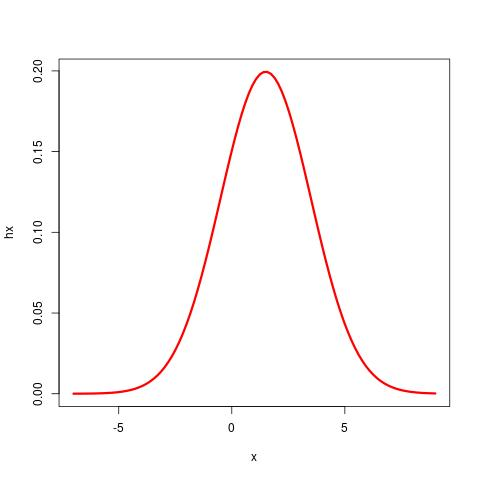
\includegraphics[width=\linewidth]{3-a}
  \caption{Sketch of $N(\frac{3}{2}, 2)$.}
  \label{fig:3-a}
\end{figure}

Sketch of the distribution can ben seen in figure \ref{fig:3-a}.

\subsection*{b.}

\[
    P(\theta = 1 \mid y = 1) = \frac{P(y=1 \mid \theta = 1) P(\theta=1)}{P(y=1)}
\]

Calculated with R:

\begin{verbatim}
> sigma = 2
> mu1 = 1
> mu2 = 2
> (pnorm(1, mu1, sigma)*1/2)/(pnorm(1, mu1, sigma)*1/2 + pnorm(1, mu2, sigma)*1/2)
[1] 0.6184005
\end{verbatim}

\subsection*{c.}

When $\sigma$ increases the data is more spread out. Therefore the probability of the distribution with mean 1 drops and the probability of the distribution with mean 2 rises. When $\sigma$ is large enough the probabilities of both distributions are getting close to 0.5.

And vice versa, if $\sigma$ decreases then the data is less spread out and therefore the probability of the distribution with mean 1 rises. When $\sigma$ is small enough it's the probability of distribution with mean 1 is getting close to 1.

This is illustrated in figure \ref{fig:3-c}.

\begin{figure}[ht!]
  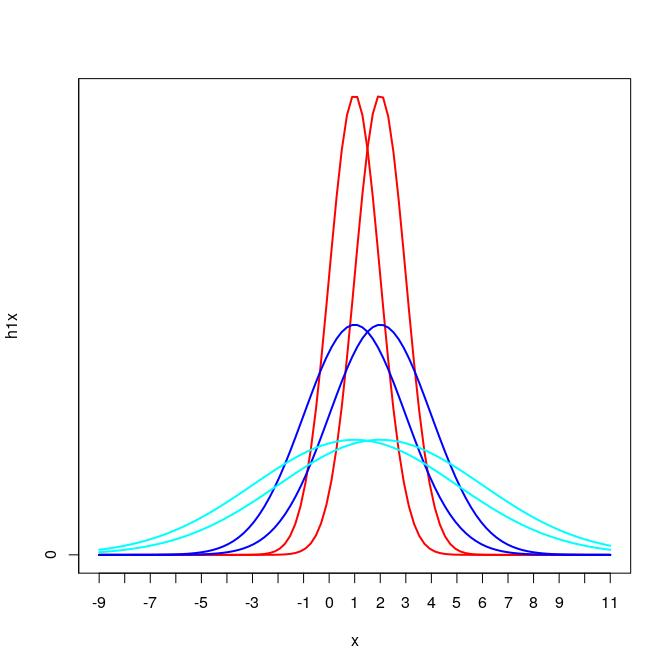
\includegraphics[width=\linewidth]{3-c}
  \caption{Normal distributions with $\mu = 1$ and $\mu = 2$. Red line has std of 1. Blue line has std of 2. Cyan line has std of 4.}
  \label{fig:3-c}
\end{figure}

\end{document}
